\documentclass[UTF8,a4paper,10pt]{ctexart}
\usepackage[left=2.50cm, right=2.50cm, top=2.50cm, bottom=2.50cm]{geometry}
%页边距
\CTEXsetup[format={\Large\bfseries}]{section} %设置章标题居左

%%%%%%%%%%%%%%%%%%%%%%%
% -- text font --
% compile using Xelatex
%%%%%%%%%%%%%%%%%%%%%%%
% -- 中文字体 --
%\setmainfont{Microsoft YaHei}  % 微软雅黑
%\setmainfont{YouYuan}  % 幼圆    
%\setmainfont{NSimSun}  % 新宋体
%\setmainfont{KaiTi}    % 楷体
%\setmainfont{SimSun}   % 宋体
%\setmainfont{SimHei}   % 黑体
% -- 英文字体 --
%\usepackage{times}
%\usepackage{mathpazo}
%\usepackage{fourier}
%\usepackage{charter}

%\usepackage{helvet}

\usepackage{amsmath, amsfonts, amssymb} % math equations, symbols
\usepackage[english]{babel}
\usepackage{color}	% color content
\usepackage{graphicx}	% import figures
\usepackage{url}	% hyperlinks
\usepackage{bm} 	% bold type for equations
\usepackage{multirow}
\usepackage{booktabs}
\usepackage{epstopdf}
\usepackage{epsfig}
\usepackage{algorithm}
\usepackage{algorithmic}
\usepackage{listings}
\usepackage{xcolor}
\usepackage{booktabs}
\usepackage{zhnumber}
\usepackage{longtable}
\usepackage{subfigure}
\usepackage{float}
\usepackage{caption}
\usepackage{subfigure}
\renewcommand\thesection{\zhnum{section}}
\renewcommand \thesubsection {\arabic{section}}
\renewcommand{\algorithmicrequire}{ \textbf{Input:}}
% use Input in the format of Algorithm  
\renewcommand{\algorithmicensure}{ \textbf{Initialize:}}
% use Initialize in the format of Algorithm  
\renewcommand{\algorithmicreturn}{ \textbf{Output:}}
% use Output in the format of Algorithm  
%%%%%%%%%%%%%%%%%%
\usepackage{listings}
\usepackage{color}
\definecolor{dkgreen}{rgb}{0,0.6,0}
\definecolor{gray}{rgb}{0.5,0.5,0.5}
\definecolor{mauve}{rgb}{0.58,0,0.82}
\lstset{frame=tb,
  language=Python,
  aboveskip=3mm,
  belowskip=3mm,
  showstringspaces=false,
  columns=flexible,
  basicstyle={\small\ttfamily},
  numbers=left,%设置行号位置none不显示行号
  %numberstyle=\tiny\courier, %设置行号大小
  numberstyle=\tiny\color{gray},
  keywordstyle=\color{blue},
  commentstyle=\color{dkgreen},
  stringstyle=\color{mauve},
  breaklines=true,
  breakatwhitespace=true,
  escapeinside=``,%逃逸字符(1左面的键),用于显示中文例如在代码中`中文...`
  tabsize=4,
  extendedchars=false %解决代码跨页时,章节标题,页眉等汉字不显示的问题
}

%%%%%%%%%%%%%%%%%%%%%%%%%%%%
\usepackage{fancyhdr} %设置页眉、页脚
\pagestyle{fancy}
\lhead{}
\chead{}
%\rhead{\includegraphics[width=1.2cm]{fig/ZJU_BLUE.eps}}
\lfoot{}
\cfoot{}
\rfoot{}
\fancyfoot[RE,RO]{~\thepage~}

\fancyhead[RE,RO]{计算物理导论 \quad 2022春季学期 \quad 作业13 \quad 何翼成}

%%%%%%%%%%%%%%%%%%%%%%%
%  设置水印
%%%%%%%%%%%%%%%%%%%%%%%
%\usepackage{draftwatermark}         % 所有页加水印
%\usepackage[firstpage]{draftwatermark} % 只有第一页加水印
% \SetWatermarkText{Water-Mark}           % 设置水印内容
% \SetWatermarkText{\includegraphics{fig/ZJDX-WaterMark.eps}}         % 设置水印logo
% \SetWatermarkLightness{0.9}             % 设置水印透明度 0-1
% \SetWatermarkScale{1}                   % 设置水印大小 0-1    

\usepackage{hyperref} %bookmarks
\hypersetup{colorlinks, bookmarks, unicode} %unicode

\title{\textbf{蒙特卡洛方法求解Ising模型(二)}}
\author{ 何翼成 \thanks{学号:520072910043; \newline
    邮箱地址:heyicheng@sjtu. edu. cn} }
\date{\today}

\begin{document}
\maketitle

%\begin{abstract}
%这是一篇中文小论文。这个部分用来写摘要。摘要的章标题默认是英文,还没找到改成中文的方法:(
%\end{abstract}
\section*{Project 1}
\section{题目分析}
%%%以下为插入图片模板
%\quad \newline
	\begin{figure}[!htbp]
		\centering
		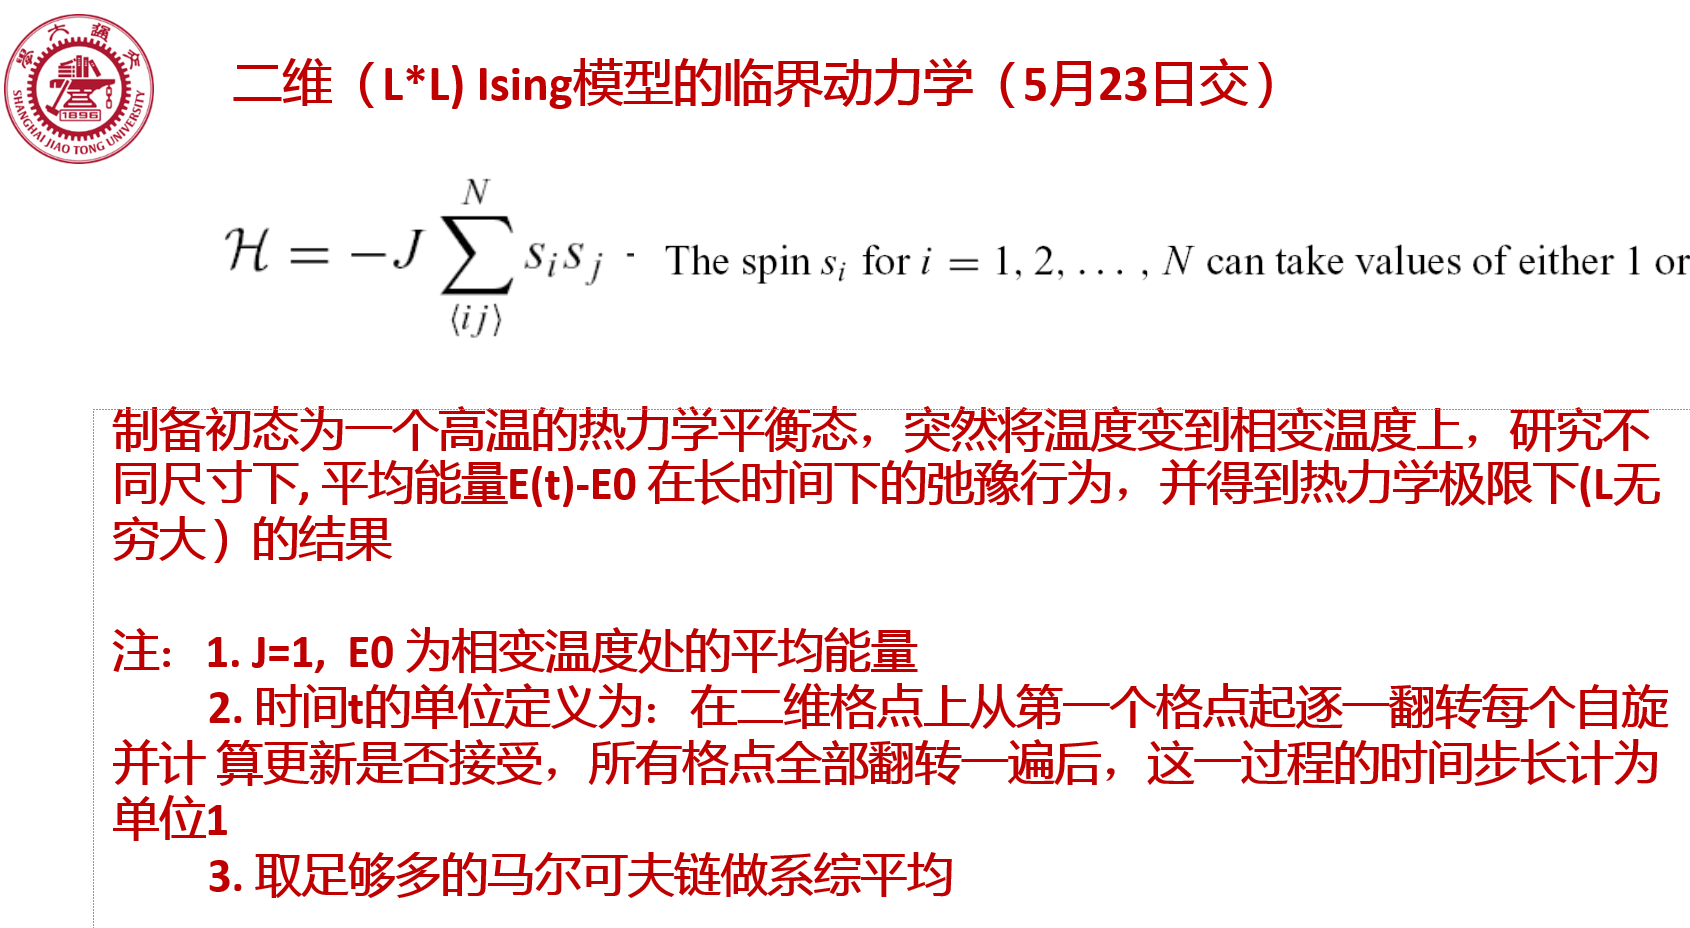
\includegraphics[width=1\textwidth,height=0.6\textwidth]{pictures/pro.png}
		\caption{题目总览} \label{project1}
	\end{figure}



\section{代码展示}
\lstset{language=matlab}
\begin{lstlisting}
    %创建方格矩阵
    Ls=[50];Tspan=linspace(100,100,2000);T0=2.269;num=800;Num=3e4;%计算步数
    A=zeros(length(Ls),num);%储存不同L下的能量-时间曲线
    for in=1:length(Ls)
        L=Ls(in);
        c=cputime;
        %设定初态的温度
        for tn=1:length(Tspan)
            T=Tspan(tn);
            Es=zeros(length(Tspan),num);
            %得到高温的热力学平衡态
            %确认尺寸,生成随机矩阵
            M=randi([0,1],L,L)*2-1;
            %逐行扫描元素,完全扫描整个矩阵为一个时间单位
            %演化num步数
            for tt=1:num
                for jj=1:L     %y
                    for ii=1:L %x
                        M_1=M;%保留磁矩矩阵的原信息
                        M_2=M;M_2(ii,jj)=-M_1(ii,jj);%翻转后的磁矩矩阵
                        pudM=pud(M);
                        deltaE=2*M(ii,jj)*(pudM(ii+2,jj+1)+pudM(ii,jj+1)+pudM(ii+1,jj+2)+pudM(ii+1,jj));
                        %判断状态是否保留
                        flag=Metro(deltaE,T0);
                        if flag==1
                            M=M_2;
                        else
                            M=M_1;
                        end
                    end
                end
            Es(tn,tt)=H(M);%计算一次能量并且储存
            cc=cputime; 
            disp("计算长度为"+L+",温度进度为"+tn/length(Tspan)*100+"%,已完成进度"+tt/num*100+"%,已耗时"+num2str((cc-c))+"s,预计用时"+(cc-c)/60/(tn/length(Tspan))+"min")
            end
        end
        Eavg=sum(Es)/length(Tspan);
        A(in,:)=Eavg;
    end
        
    %计算T0时的平均能量
        E0=AverageH(L,T,Num,10);
        plot(1:num,A-E0)
        legend("L="+L)
        xlabel("LogTime")
        ylabel("Log(E-E_{0})")
    
    %%
    %Metropolis算法函数的定义
    function flag=Metro(deltaE,T)
        beta=1/T;
        if deltaE<=0
            p=1;
        else
            p=exp(-beta*deltaE);
        end
        z=rand();
        if z<p
           flag=1;
        else
            flag=0;
        end
    end
    %%
    %Pud,辅助计算。扩展为(L+2)**2的矩阵
    function pudM=pud(M)
    L=size(M,1);
    pudM=zeros(L+2,L+2);%分配储存空间
    %pudding,采用周期性边界条件
    pudM(2:(L+1),2:(L+1))=M;
    %行的移动
    pudM(1,2:(L+1))=M(L,:);
    pudM(L+2,2:(L+1))=M(1,:);
    %列的移动
    pudM(2:(L+1),1)=M(:,L);
    pudM(2:(L+1),L+2)=M(:,1);
    end
    
    %能量计算
    function E=H(M)
    L=size(M,1);
    pudM=pud(M);
    H=0;
    for i=2:L
        for j=2:L
            H=H-pudM(i,j)*(pudM(i,j-1)+pudM(i,j+1)+pudM(i-1,j)+pudM(i+1,j));
        end
    end
    E=H/2;
    end
    
    %%
    %平均能量计算.输入尺寸,温度,循环次数,并行链条数,计算该温度下的矩阵的平均能量
    function avgH=AverageH(L,T,Num,s)
    %创建随机矩阵
    Matrix=randi([0,1],L,L)*2-1;
    %创建空数组记录能量值
    Hels=zeros(s,Num);
    for ss=1:s
    for mm=1:Num
        locs=randi([1,L],1,2);%创建随机坐标
        x=locs(1);y=locs(2);
        Matrix_1=Matrix;%保留磁矩矩阵的原信息
        Matrix_2=Matrix;Matrix_2(x,y)=-Matrix_1(x,y);%翻转后的磁矩矩阵
        pudMatrix=pud(Matrix);
        deltaE=2*Matrix(x,y)*(pudMatrix(x+2,y+1)+pudMatrix(x,y+1)+pudMatrix(x+1,y+2)+pudMatrix(x+1,y));
        %判断状态是否保留
        flag=Metro(deltaE,T);
        if flag==1
            Matrix=Matrix_2;
        else
            Matrix=Matrix_1;
        end
        Hels(ss,Num)=H(Matrix);
    end
    end
    avgH=sum(Hels,"all")/(Num*s);
    end
\end{lstlisting}

\section{结果分析与结论}
\subsubsection{原图像}
\begin{figure}[!htbp]
    \centering
    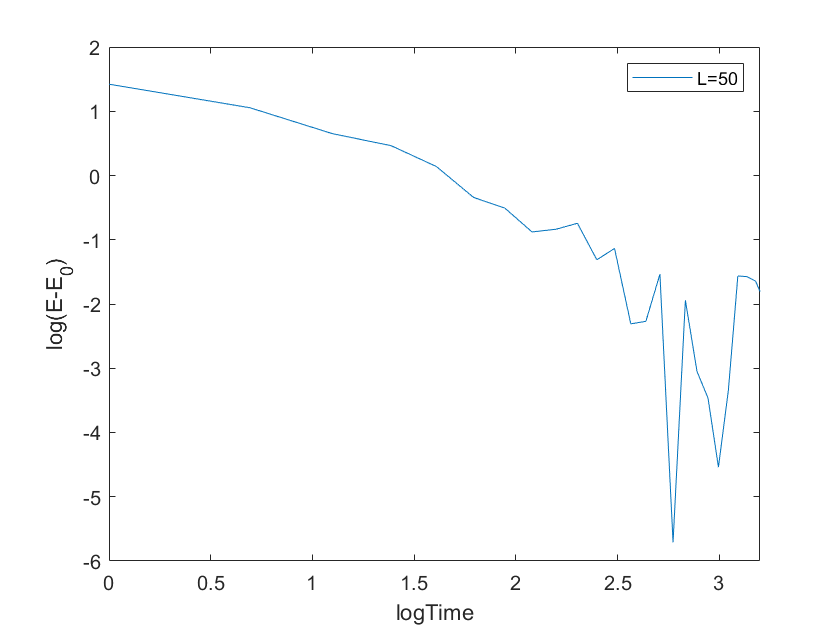
\includegraphics[width=1\textwidth,height=1\textwidth]{pictures/L50.png}
    \caption{<H>-Time with L=50}
\end{figure}
\subsubsection{取对数轴进行逼近}
\begin{figure}[!htbp]
    \centering
    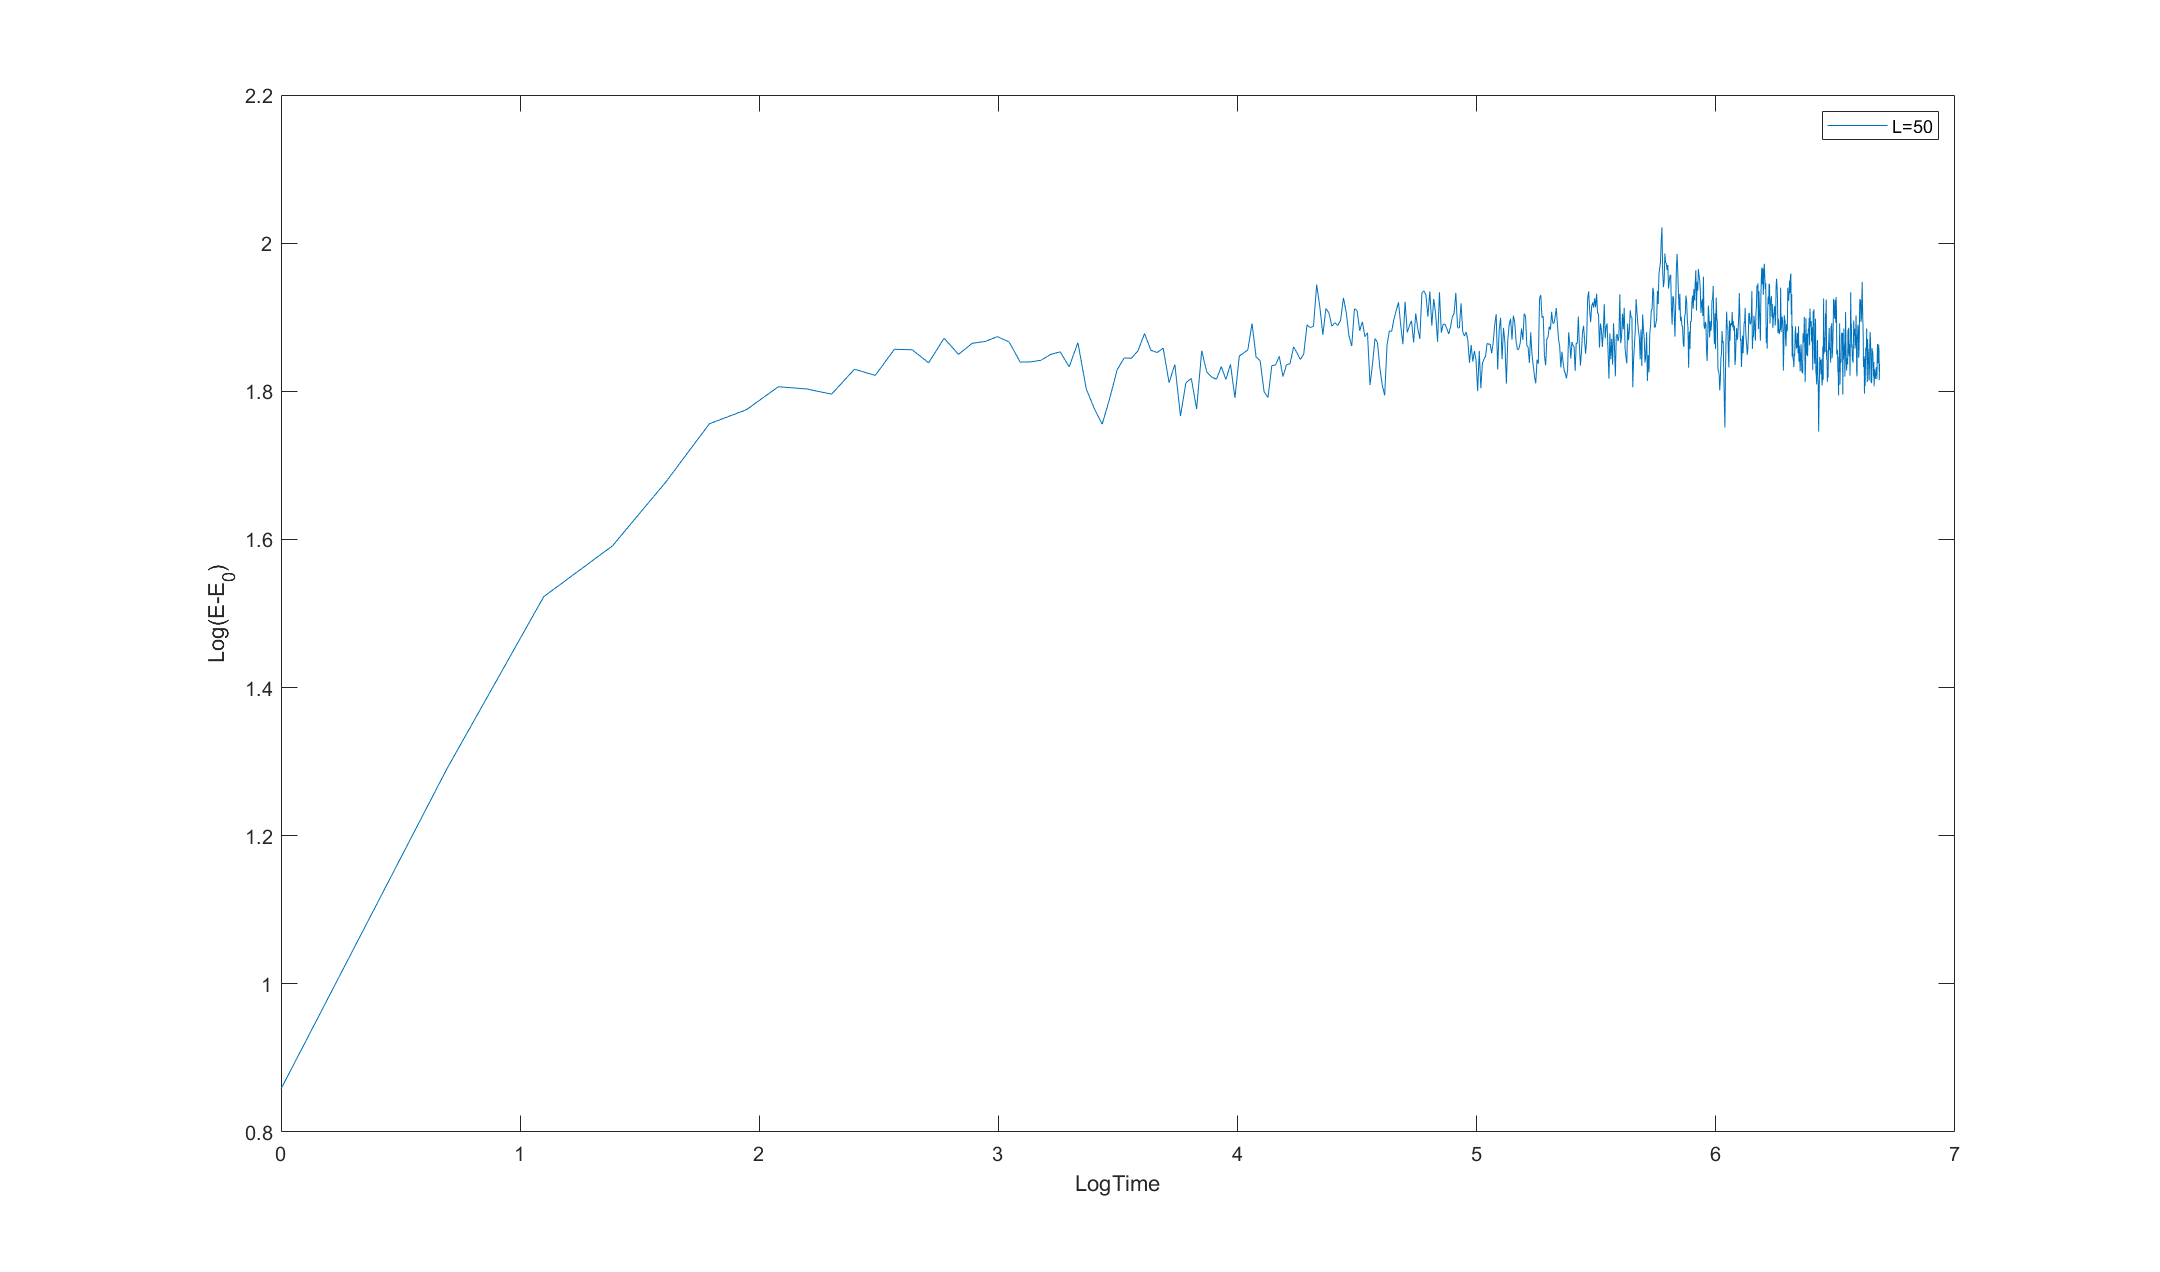
\includegraphics[width=1\textwidth,height=1\textwidth]{pictures/logL50.png}
    \caption{log<H>-logTime}
\end{figure}
由于笔记本CPU性能问题,在计算过程中即使采取了多种近似和精简方法,在L增大至50左右时,所需要的时间就开始急速增长.
所以本文中分析过程也会局限于L<50的范围.\newline

根据图像分析可知,随着L取值的增大,其图线的意义逐渐趋向于热力学极限.从原始图像来看,就是原本高温的平衡态逐渐平衡在
了$T_{0}=2.269K$.为了方便分析,我们对代表时间意义的Time轴和平均能量均取对数,从而得到了一个弯曲的曲线.
我们可以合理推论:当L趋向于无穷大时,其图线将会趋于一条直线.
%以下为插入代码模板
%~\\
%\lstset{language=matlab}
%\begin{lstlisting}
%\end{lstlisting}


%%%以下为插入图片模板
%\quad \newline
%	\begin{figure}[!htbp]
%		\centering
%		\includegraphics[width=0.5\textwidth,height=0.375\textwidth]{pictures/minscale.png}
%		\caption{最小风向} \label{minsacle}
%	\end{figure}

%%%以下为插入图片模板
%\quad \newline
%	\begin{figure}[!htbp]
%		\centering
%		\includegraphics[width=0.5\textwidth,height=0.375\textwidth]{pictures/minscale.png}
%		\caption{最小风向} \label{minsacle}
%	\end{figure}

%    \begin{algorithm}
%		\caption{Title of the Algorithm}
%     	\begin{algorithmic}[1]
%			\REQUIRE some words.  % this command shows "Input"
%			\ENSURE ~\\           % this command shows "Initialized"
%			some text goes here ... \\
%			\WHILE {\emph{not converged}}
%			\STATE ... \\  % line number at left side
%			\ENDWHILE
%			\RETURN this is the lat part.  % this command shows "Output"
%		\end{algorithmic}
%	\end{algorithm}

\end{document}